\documentclass[10pt]{beamer}\usepackage[]{graphicx}\usepackage[]{color}
% maxwidth is the original width if it is less than linewidth
% otherwise use linewidth (to make sure the graphics do not exceed the margin)
\makeatletter
\def\maxwidth{ %
  \ifdim\Gin@nat@width>\linewidth
    \linewidth
  \else
    \Gin@nat@width
  \fi
}
\makeatother

\definecolor{fgcolor}{rgb}{0.345, 0.345, 0.345}
\newcommand{\hlnum}[1]{\textcolor[rgb]{0.686,0.059,0.569}{#1}}%
\newcommand{\hlstr}[1]{\textcolor[rgb]{0.192,0.494,0.8}{#1}}%
\newcommand{\hlcom}[1]{\textcolor[rgb]{0.678,0.584,0.686}{\textit{#1}}}%
\newcommand{\hlopt}[1]{\textcolor[rgb]{0,0,0}{#1}}%
\newcommand{\hlstd}[1]{\textcolor[rgb]{0.345,0.345,0.345}{#1}}%
\newcommand{\hlkwa}[1]{\textcolor[rgb]{0.161,0.373,0.58}{\textbf{#1}}}%
\newcommand{\hlkwb}[1]{\textcolor[rgb]{0.69,0.353,0.396}{#1}}%
\newcommand{\hlkwc}[1]{\textcolor[rgb]{0.333,0.667,0.333}{#1}}%
\newcommand{\hlkwd}[1]{\textcolor[rgb]{0.737,0.353,0.396}{\textbf{#1}}}%
\let\hlipl\hlkwb

\usepackage{framed}
\makeatletter
\newenvironment{kframe}{%
 \def\at@end@of@kframe{}%
 \ifinner\ifhmode%
  \def\at@end@of@kframe{\end{minipage}}%
  \begin{minipage}{\columnwidth}%
 \fi\fi%
 \def\FrameCommand##1{\hskip\@totalleftmargin \hskip-\fboxsep
 \colorbox{shadecolor}{##1}\hskip-\fboxsep
     % There is no \\@totalrightmargin, so:
     \hskip-\linewidth \hskip-\@totalleftmargin \hskip\columnwidth}%
 \MakeFramed {\advance\hsize-\width
   \@totalleftmargin\z@ \linewidth\hsize
   \@setminipage}}%
 {\par\unskip\endMakeFramed%
 \at@end@of@kframe}
\makeatother

\definecolor{shadecolor}{rgb}{.97, .97, .97}
\definecolor{messagecolor}{rgb}{0, 0, 0}
\definecolor{warningcolor}{rgb}{1, 0, 1}
\definecolor{errorcolor}{rgb}{1, 0, 0}
\newenvironment{knitrout}{}{} % an empty environment to be redefined in TeX

\usepackage{alltt}


%\input{slides_header.tex}
\usepackage{graphicx}
\usepackage{hyperref, url}
\hypersetup{colorlinks,citecolor=myorange,filecolor=red,linkcolor=brown,urlcolor=blue}

\usepackage{longtable,booktabs}
\usepackage{amssymb,amsmath}
\usepackage{animate}
\usepackage{subfig}
\usepackage{tikz}
\usetikzlibrary{shapes.geometric, arrows,shapes.symbols,decorations.pathreplacing}
\tikzstyle{startstop} = [rectangle, rounded corners, minimum width=3cm, minimum height=1cm, draw=black, fill=pinkish,text width=3.5cm]
\tikzstyle{startstop2} = [rectangle, rounded corners, minimum width=3cm, minimum height=1cm, draw=black, fill=background,text width=4.5cm]
\tikzstyle{startstop3} = [rectangle, rounded corners, minimum width=3cm, minimum height=1cm, draw=black, fill=beige,text width=3.0cm]
\tikzstyle{startstop4} = [rectangle, rounded corners, minimum width=3cm, minimum height=1cm, draw=black, fill=pinkish,text width=4.5cm]
\tikzstyle{io} = [trapezium, trapezium left angle=70, trapezium right angle=110, minimum width=2cm, minimum height=1cm, text centered, draw=black, fill=blue!30,text width=1.5cm]
\tikzstyle{process} = [rectangle, minimum width=1cm, minimum height=1cm, text centered, draw=black, fill=orange!30,text width=2cm]
\tikzstyle{decision} = [diamond, minimum width=2cm, minimum height=1cm, text centered, draw=black, fill=green!30]
\tikzstyle{arrow} = [thick,->,>=stealth]
\tikzstyle{both} = [thick,<->,>=stealth, red]


% used for tree of stats tests in 001-introduction
\tikzstyle{startstopstats} = [rectangle, rounded corners, minimum width=2cm, minimum height=.5cm,text centered, draw=black, fill=red!30]
\tikzstyle{iostats} = [trapezium, trapezium left angle=70, trapezium right angle=110, minimum width=2cm, minimum height=.5cm, text centered, draw=black, fill=blue!30]
\tikzstyle{processstats} = [rectangle, minimum width=1.5cm, minimum height=.5cm, text centered, draw=black, fill=orange!30]
\tikzstyle{processbigstats} = [rectangle, minimum width=1.5cm, minimum height=.5cm, text centered, draw=black, fill=orange!30,text width=1.6cm]
\tikzstyle{decisionstats} = [rectangle, minimum width=1cm, minimum height=1cm, text centered, draw=black, fill=green!30,text width=1.6cm]
\tikzstyle{decisionbigstats} = [rectangle, minimum width=1cm, minimum height=1cm, text centered, draw=black, fill=yellow!30,text width=2cm]

\usepackage{pifont}% http://ctan.org/pkg/pifont
\newcommand{\cmark}{\ding{51}}%
\newcommand{\xmark}{\ding{55}}%

\usepackage{ulem} % for strikeout

\usepackage{xcolor}
\usepackage{color, colortbl}
\definecolor{lightgray}{RGB}{200,200,200}
\definecolor{palegray}{RGB}{221,221,221}
\definecolor{myblue}{RGB}{0,89,179}
\definecolor{myorange}{rgb}{0.776,0.357,0.157}
\definecolor{gray}{RGB}{110,110,110}
\definecolor{darkgray}{RGB}{100,100,100}
\definecolor{lightgray}{RGB}{200,200,200}
\definecolor{palegray}{RGB}{221,221,221}
\definecolor{turquoise}{RGB}{81,193,188}
\definecolor{tomato}{RGB}{255,136,136}
\definecolor{mandarina}{RGB}{229,169,25}
\definecolor{foreground}{RGB}{81,141,193}
\definecolor{background}{RGB}{246,244,240}
\definecolor{highlight}{RGB}{229,169,25}
\definecolor{lowlight}{RGB}{200,200,200}
\definecolor{beige}{RGB}{255,255,240}
\definecolor{pinkish}{RGB}{255,223,247}
\definecolor{darktangerine}{rgb}{1.0, 0.66, 0.07}
\definecolor{deepink}{RGB}{255,20,147}
%\usepackage{shadethm}
%\colorlet{shadecolor}{blue!15}
%\colorlet{shadecolor}{palegray}
%\setlength{\shadeboxrule}{.4pt}

%\newshadetheorem{thm}{Theorem}
%\newshadetheorem{defm}{Definition}
%\newshadetheorem{exm}{Exercise}
%\newshadetheorem{remarkm}{Remark}
%\definecolor{shadethmcolor}{HTML}{EDF8FF}
%\definecolor{shadethmcolor}{RGB}{221,221,221}
%\definecolor{shaderulecolor}{HTML}{45CFFF}
%\definecolor{shaderulecolor}{RGB}{0,89,179}
%\setlength{\shadeboxrule}{.4pt}



\usepackage{epsfig}

\newcommand{\code}[1]{\texttt{#1}}
\newcommand{\blue}[1]{\textcolor{blue}{#1}}
\newcommand{\red}[1]{\textcolor{red}{#1}}

\usepackage{comment}

\makeatletter

\def \iqsssectiontitleheader {}

\newcommand{\iqsssectiontitle}[1]{
	\def \iqsssectiontitleheader{#1}
}

\@ifundefined{insertmainframenumber}
{%
	% \insertmainframenumber not defined
	\newcommand{\insertmainframenumber}{\inserttotalframenumber}
}
{%
	% \insertmainframenumber already defined
}%


\AtBeginSection[]{
	\title{\insertsectionhead}
	{
		%\definecolor{white}{RGB}{140,193,250}
		%\definecolor{white}{RGB}{200,200,200}
		%\definecolor{white}{RGB}{242,244,247}
		\definecolor{white}{RGB}{0,89,179}
		%\definecolor{iqss@orange}{rgb}{1,1,1}
		\ifnum \insertmainframenumber > \insertframenumber
		%\setbeamercolor{background canvas}{bg=myblue}
		%\setbeamercolor{normal text}{fg=black,bg=white}
		%\setbeamercolor{frametitle}{fg=red}
		%\setbeamercolor{section in toc}{fg=myblue, bg=white}
		%\setbeamercolor{subsection in toc}{fg=myblue, bg=white}
		\frame{
			\frametitle{\iqsssectiontitleheader}
			\tableofcontents[currentsection]
		}
		\else
		\frame{
			\frametitle{Backup Slides}
			\tableofcontents[sectionstyle=shaded/shaded,subsectionstyle=shaded/shaded/shaded]
		}
		\fi
	}
}
\makeatother
%\graphicspath{{/home/sahir/git_repositories/EPIB607/resources/assets/slides/figure/}}


\usepackage{fontspec}
%\setsansfont{Fira Sans}
%\setmonofont{Fira Mono}
%\setsansfont[ItalicFont={Fira Sans Light Italic},BoldFont={Fira Sans},BoldItalicFont={Fira Sans Italic}]{Fira Sans Light}
%\setmonofont[BoldFont={Fira Mono Medium}]{Fira Mono}

\def\installpath{/usr/local/share/texmf/fonts/opentype/libertinus/}
\setmainfont{LibertinusSerif}[
UprightFont    = *-Regular,
BoldFont       = *-Bold,
ItalicFont     = *-Italic,
BoldItalicFont = *-BoldItalic,
Ligatures      = TeX,
Extension      = .otf,
Path           = \installpath/
]

\setsansfont{LibertinusSerif}[
UprightFont    = *-Regular,
BoldFont       = *-Bold,
ItalicFont     = *-Italic,
BoldItalicFont = *-BoldItalic,
Ligatures      = TeX,
Extension      = .otf,
Path           = \installpath/
]


%\setmonofont{LibertinusSerif}[
%UprightFont    = *-Regular,
%BoldFont       = *-Bold,
%ItalicFont     = *-Italic,
%BoldItalicFont = *-BoldItalic,
%Ligatures      = TeX,
%Extension      = .otf,
%Path           = \installpath/
%]






\newcommand\Wider[2][3em]{%
	\makebox[\linewidth][c]{%
		\begin{minipage}{\dimexpr\textwidth+#1\relax}
			\raggedright#2
		\end{minipage}%
	}%
}


\newcommand {\framedgraphic}[1] {
	\begin{figure}
		\centering
		\includegraphics[width=\textwidth,height=0.9\textheight,keepaspectratio]{#1}
	\end{figure}
}


\newcommand {\framedgraphiccaption}[2] {
	\begin{figure}
		\centering
		\includegraphics[width=\textwidth,height=0.8\textheight,keepaspectratio]{#1}
		\caption{#2}
	\end{figure}
}




\setbeamercolor{itemize item}{fg=myblue}
\setbeamercolor{itemize subitem}{fg=myorange}
%\setbeamertemplate{itemize item}[square]
\setbeamertemplate{itemize item}[circle]
\setbeamertemplate{itemize subitem}[triangle]
\setbeamertemplate{blocks}[rounded][shadow=true]
\setbeamercolor{block body alerted}{bg=alerted text.fg!10}
\setbeamercolor{block title alerted}{bg=alerted text.fg!20}
\setbeamercolor{block body}{bg=structure!10}
\setbeamercolor{block title}{bg=structure!20}
\setbeamercolor{block body example}{bg=green!10}
\setbeamercolor{block title example}{bg=green!20}


\makeatletter
\newenvironment<>{proofs}[1][\proofname]{%
	\par
	\def\insertproofname{#1\@addpunct{.}}%
	\usebeamertemplate{proof begin}#2}
{\usebeamertemplate{proof end}}
\newenvironment<>{proofc}{%
	\setbeamertemplate{proof begin}{\begin{block}{}}
		\par
		\usebeamertemplate{proof begin}}
	{\usebeamertemplate{proof end}}
	\newenvironment<>{proofe}{%
		\par
		\pushQED{\qed}
		\setbeamertemplate{proof begin}{\begin{block}{}}
			\usebeamertemplate{proof begin}}
		{\popQED\usebeamertemplate{proof end}}
\makeatother


\makeatletter
\newenvironment<>{exams}[1][\proofname]{%
	\par
	\def\insertproofname{#1\@addpunct{.}}%
	\usebeamertemplate{example begin}#2}
{\usebeamertemplate{example end}}
\newenvironment<>{examc}{%
	\setbeamertemplate{exam begin}{\begin{block}{}}
		\par
		\usebeamertemplate{exam begin}}
	{\usebeamertemplate{exam end}}
	\newenvironment<>{exame}{%
		\par
		\pushQED{\qed}
		\setbeamertemplate{exam begin}{\begin{block}{}}
			\usebeamertemplate{exam begin}}
		{\popQED\usebeamertemplate{exam end}}
		\makeatother

%\definecolor{mycolor}{HTML}{F7F8E0}
%\declaretheorem[shaded={bgcolor=mandarina}]{theo}
%\declaretheorem[shaded={bgcolor=mycolor}]{propo}
%\declaretheorem[shaded={bgcolor=green!80!black!30}]{remark}

%\setbeamertemplate{navigation symbols}{\usebeamercolor[fg]{title in head/foot}\usebeamerfont{title in head/foot}\insertframenumber}


%\setbeamertemplate{footline}{}

\beamertemplatenavigationsymbolsempty % toggle off if you want navigation symbols at the bottom

\setbeamertemplate{footline}
{ \usebeamercolor[fg]{page number in head/foot}%
	\usebeamerfont{page number in head/foot}%
	\hspace{1em}\insertsectionhead%
	\hfill%
	\insertframenumber\,/\,\hyperlinkappendixstart{\insertmainframenumber}
	\ifnum \thepage = \insertframeendpage{\small .}\else{\phantom{\small .}}\fi
	\hspace{1em}
	\vskip2pt%
}

%\newtheorem{proposition}[theorem]{Proposition}
%\newtheorem{exercise}[theorem]{Exercise}
%\newtheorem{remark}[theorem]{Remark}


\usepackage{amsthm}
\usepackage{thmtools}

\setbeamertemplate{theorems}[ams style] 
%\setbeamertemplate{theorems}[numbered] 
%\setbeamertemplate{corollary}[numbered] 
\newtheorem{proposition}{Proposition}
\newtheorem{exercise}{Exercise}
\newtheorem{remark}{Remark}
\newtheorem{exam}{Example}
%\newtheorem{proof}{Proof}
%\newtheorem{corollaries}[theorem]{Corollary}
\newcommand*{\theorembreak}{\usebeamertemplate{theorem end}\framebreak\usebeamertemplate{theorem begin}}



\setlength{\emergencystretch}{3em} % prevent overfull lines
\providecommand{\tightlist}{%
	\setlength{\itemsep}{0pt}\setlength{\parskip}{0pt}}

\newcommand\AddButton{%
	\setbeamertemplate{background canvas}{%
		\begin{tikzpicture}[remember picture,overlay]
		\node[anchor=west] at ([yshift=5pt,xshift=0.1em]current page.south west)
		{\hyperlink{toc}{\beamergotobutton{back to TOC}}};
		\end{tikzpicture}%
	}%
}


\titlegraphic{\hfill
\includegraphics[height=1cm]{/home/sahir/git_repositories/EPIB607/slides/mcgill_logo.png}}




\graphicspath{{/home/sahir/git_repositories/EPIB607/slides/figure/}}

%\let\oldShaded\Shaded
%\let\endoldShaded\endShaded
%\renewenvironment{Shaded}{\footnotesize\oldShaded}{\endoldShaded}
\IfFileExists{upquote.sty}{\usepackage{upquote}}{}
\begin{document}



%\title{Introduction to Regression Trees}
%\author{Sahir Bhatnagar \inst{1}}
%\author[shortname]{Sahir Rai Bhatnagar, PhD Candidate (Biostatistics) }
%\institute[shortinst]{Department of Epidemiology, Biostatistics and Occupational Health}

	\title{009 - Confidence Intervals}
\author{EPIB 607 - FALL 2020}
\institute{
	Sahir Rai Bhatnagar\\
	Department of Epidemiology, Biostatistics, and Occupational Health\\
	McGill University\\
	
	\vspace{0.1 in}
	
	\texttt{sahir.bhatnagar@mcgill.ca}\\
	%\texttt{\url{https://sahirbhatnagar.com/EPIB607/}}
}

\date{slides compiled on \today}

\maketitle

\begin{frame}{Key takeaways and next steps}
	\begin{enumerate}
		\setlength\itemsep{2em}
		\item We've been exclusively talking about point estimates \pause
		\item How confident are we about these point estimates? \pause
		\item \textcolor{blue}{Thought experiment}: Estimate the average temperature in Montreal in August over the past 100 years. How much money would you be willing to bet on it?\pause  
		\item We're going into stat territory now. 
	\end{enumerate}
\end{frame}



%\section{Parameter Intervals}


\section{Reverse engineering logic}

\subsection{Example 1: Height of a building}

\begin{frame}{Example 1: Height of a building}
\begin{itemize}
	\item Consider the height of a particular building \(\theta\).
	\item We use tools of mathematical science (trignometry) to	measure it. 	
\item Suppose you measure the height of this building by standing a known horizontal distance (e.g. 100 metres) from the bottom of the building	and using an instrument to measure the angle between the horizontal and the top of the building.
\end{itemize}
\end{frame}




\begin{frame}[fragile,plain]
	
\begin{knitrout}\tiny
\definecolor{shadecolor}{rgb}{0.969, 0.969, 0.969}\color{fgcolor}

{\centering 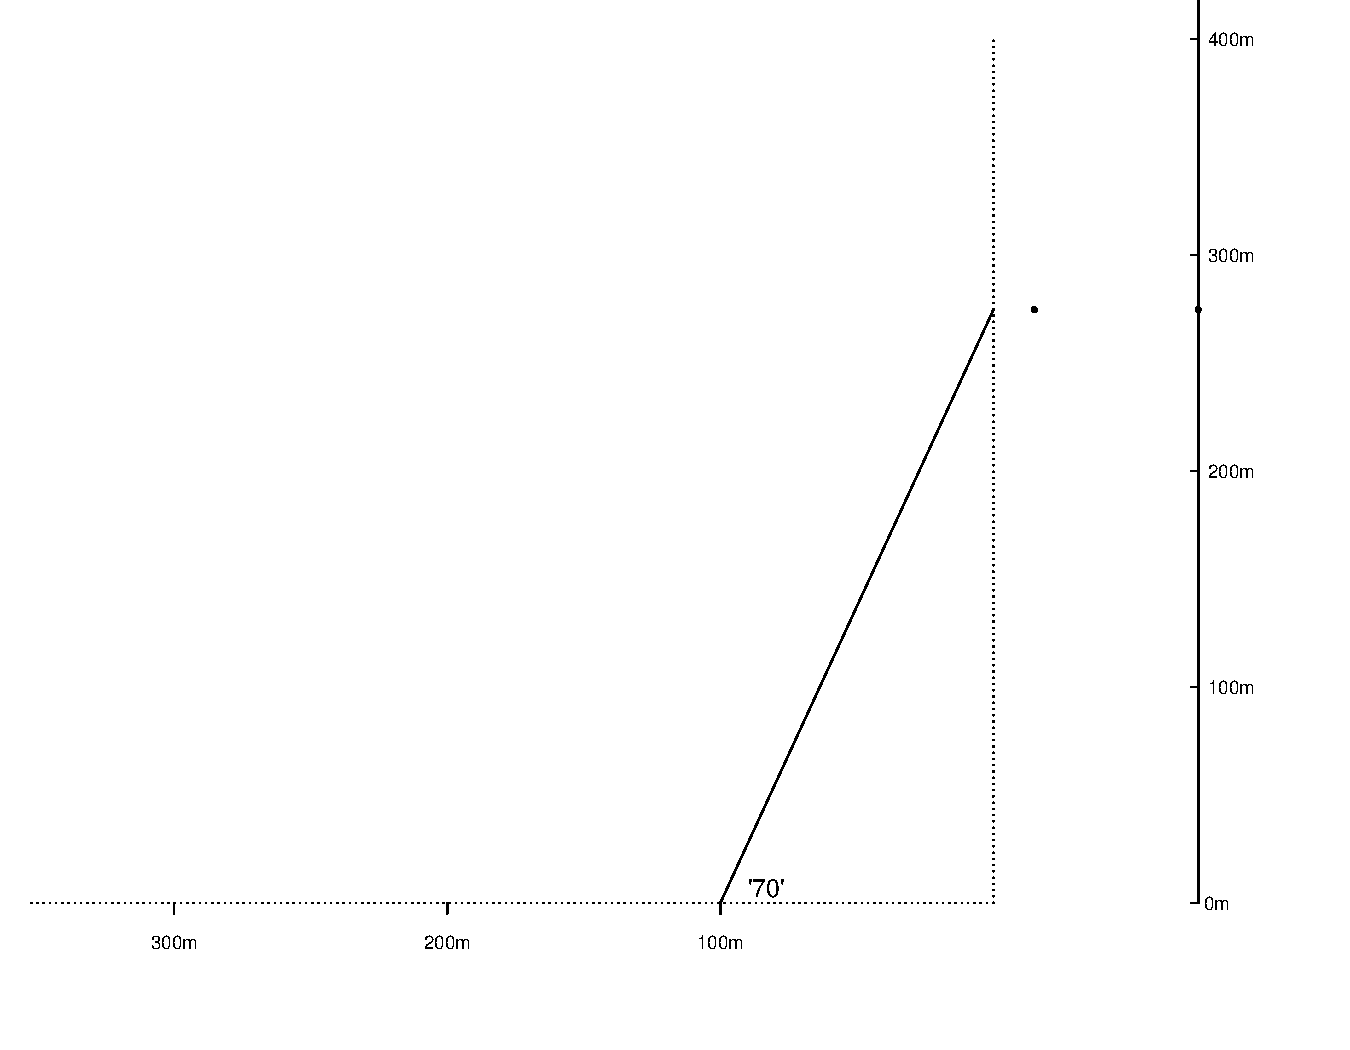
\includegraphics[width=\maxwidth]{figure/hanley-fig3-1} 

}



\end{knitrout}
	
	
\end{frame}


\begin{frame}{Example 1: Height of a building}
	\begin{itemize}
		\item After calculating this, you learn that the measuring instrument only
		displays the angle is to the nearest 10 degrees. This means that the
		true angle is somewhere between 65 and 75 degrees.
		
\item 		So you \textbf{cannot say} that the true height is \textbf{exactly} 275
		metres. What \textbf{can} you say? And with what certainty?
	\pause	
\item 		You can put \textbf{limits} on the true height by asking \textbf{what
			are the minimum and maximum heights that could have produced the
			observed reading of 70 degrees?}

	\end{itemize}
\end{frame}


\begin{frame}{Example 1: Height of a building}
	\begin{itemize}
		\item \textbf{Lower limit:} What is the \textbf{minimum} angle that could have given the (rounded) readout of 70 degrees ?
		
		\vspace{1in}
		
		\pause 
		
				\item \textbf{Upper limit:} What is the \textbf{maximum} angle that could have given the (rounded) readout of 70 degrees ?
		
	\end{itemize}
\end{frame}





\begin{frame}[fragile]{Example 1: Height of a building}

\begin{knitrout}\tiny
\definecolor{shadecolor}{rgb}{0.969, 0.969, 0.969}\color{fgcolor}\begin{figure}

{\centering 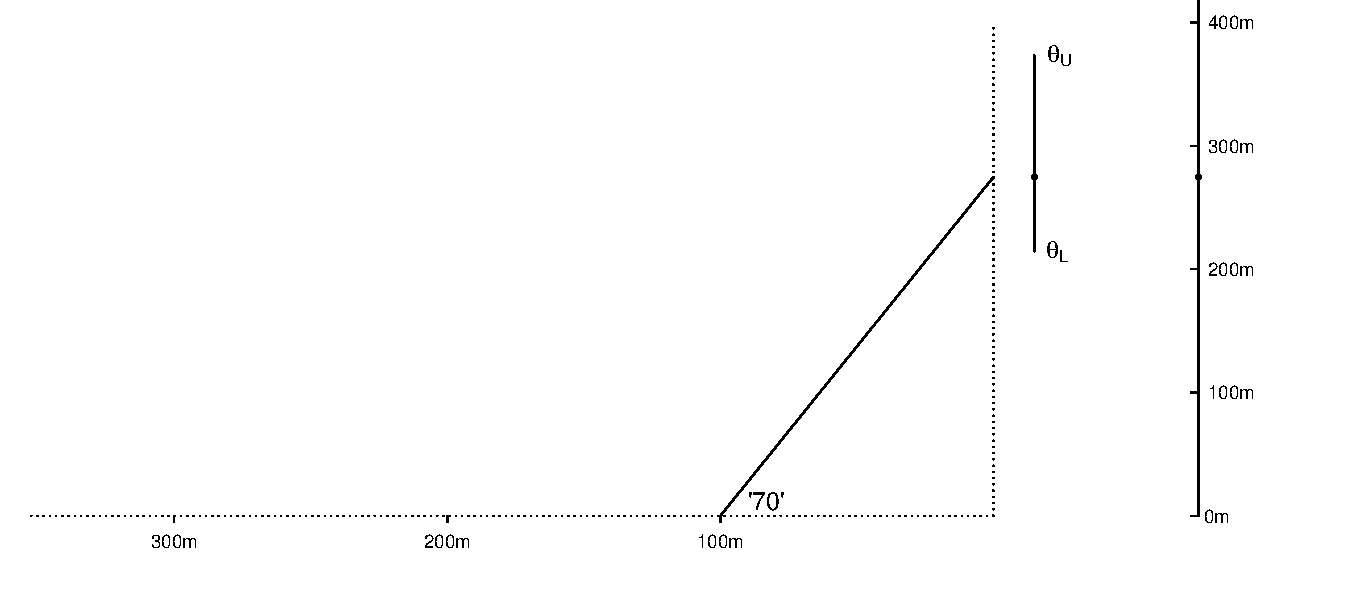
\includegraphics[width=\maxwidth]{figure/hanley-fig2-1} 

}

\caption[Estimating the height of an building by measuring subtended angles]{Estimating the height of an building by measuring subtended angles. The '70' signifies that the real angle was somewhere between 65 and 75 degrees; thus the real height lies between the L and U limits of 214 and 373 metres.}\label{fig:hanley-fig2}
\end{figure}


\end{knitrout}


\end{frame}

\subsection{Example 2: Estimating calendar age}

\begin{frame}{Example 2: Estimating calendar age\footnote{\tiny{People smugglers, statistics and bone age by Tim Cole (2012). Significance Magazine. \url{https://doi.org/10.1111/j.1740-9713.2012.00568.x}}}}
	\centering
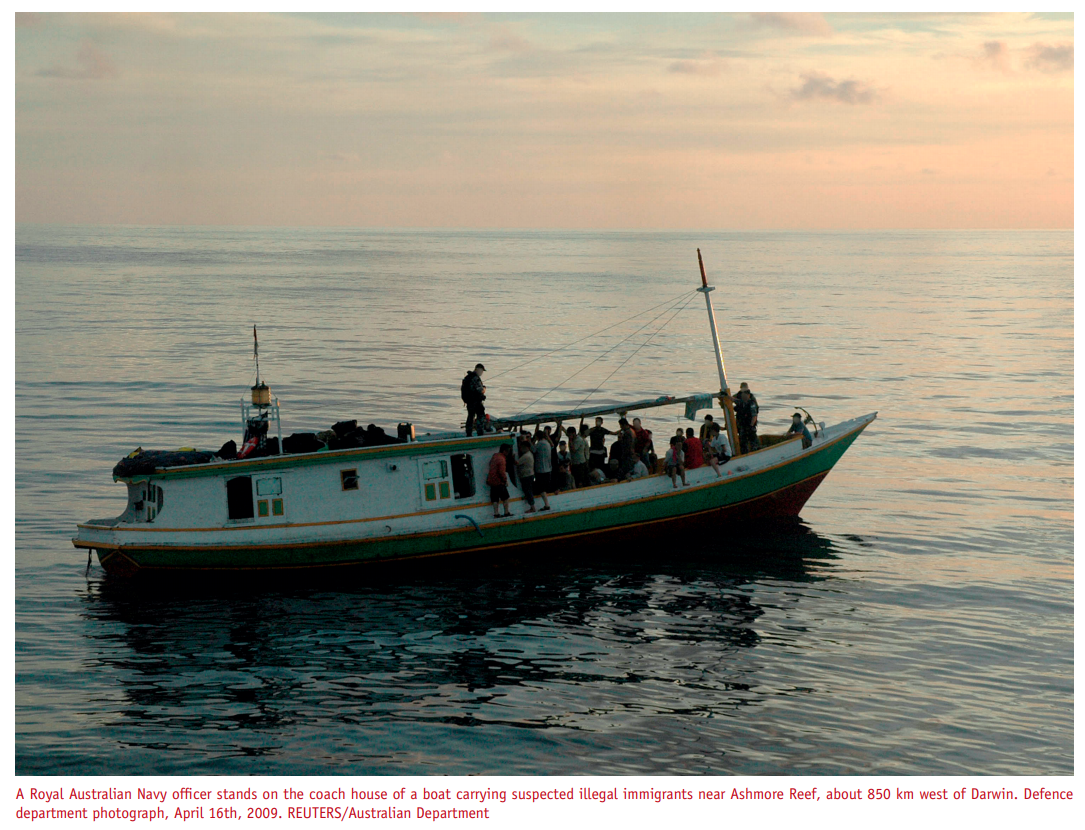
\includegraphics[scale=0.35]{boat.png}
\end{frame}


\begin{frame}{Example 2: Estimating calendar age\footnote{\tiny{People smugglers, statistics and bone age by Tim Cole (2012). Significance Magazine. \url{https://doi.org/10.1111/j.1740-9713.2012.00568.x}}}}
	\centering
	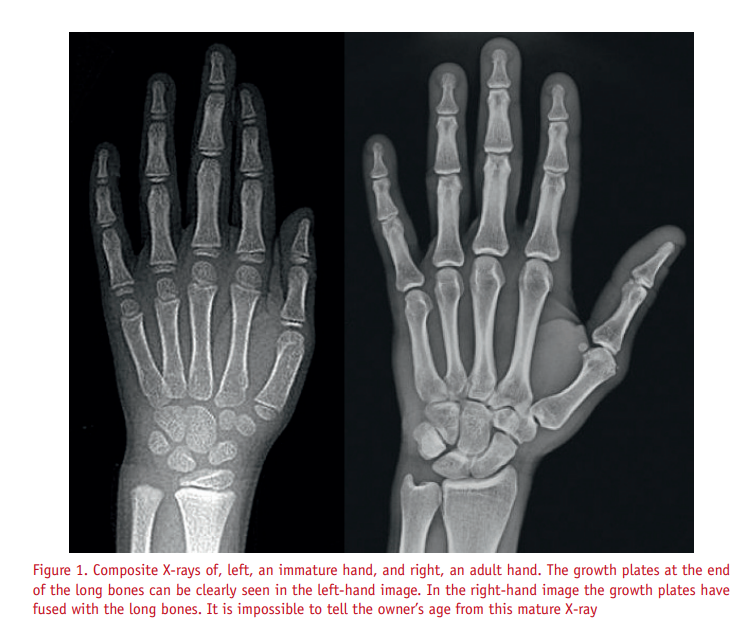
\includegraphics[scale=0.35]{xray.png}
\end{frame}


\begin{frame}{Example 2: Estimating calendar age}
\begin{itemize}
	\item The person's correct chronological age is a particularistic
	parameter, one that had nothing to do with science, or universal laws of
	Nature. But it can be estimated by using the laws of mathematics and
	statistics.
	\pause 
	
	\item Consider first a single indirect measurement of chronological age, that
	yielded a value of 17.6 years.
	
	\pause 
	
	\item Given what you know about the sizes of the possible errors, you
	\textbf{cannot say} that the true age is \textbf{exactly} 17.6 years
	What \textbf{can} you say? And with what certainty?
	
	\pause 
	
	\item You can put \textbf{limits} on the true age by asking \textbf{what are
		the minimum and maximum ages that could have produced the observed
		reading of} 17.6 years.
\end{itemize}
\end{frame}







\begin{frame}[fragile,plain]



\begin{knitrout}\tiny
\definecolor{shadecolor}{rgb}{0.969, 0.969, 0.969}\color{fgcolor}\begin{figure}

{\centering 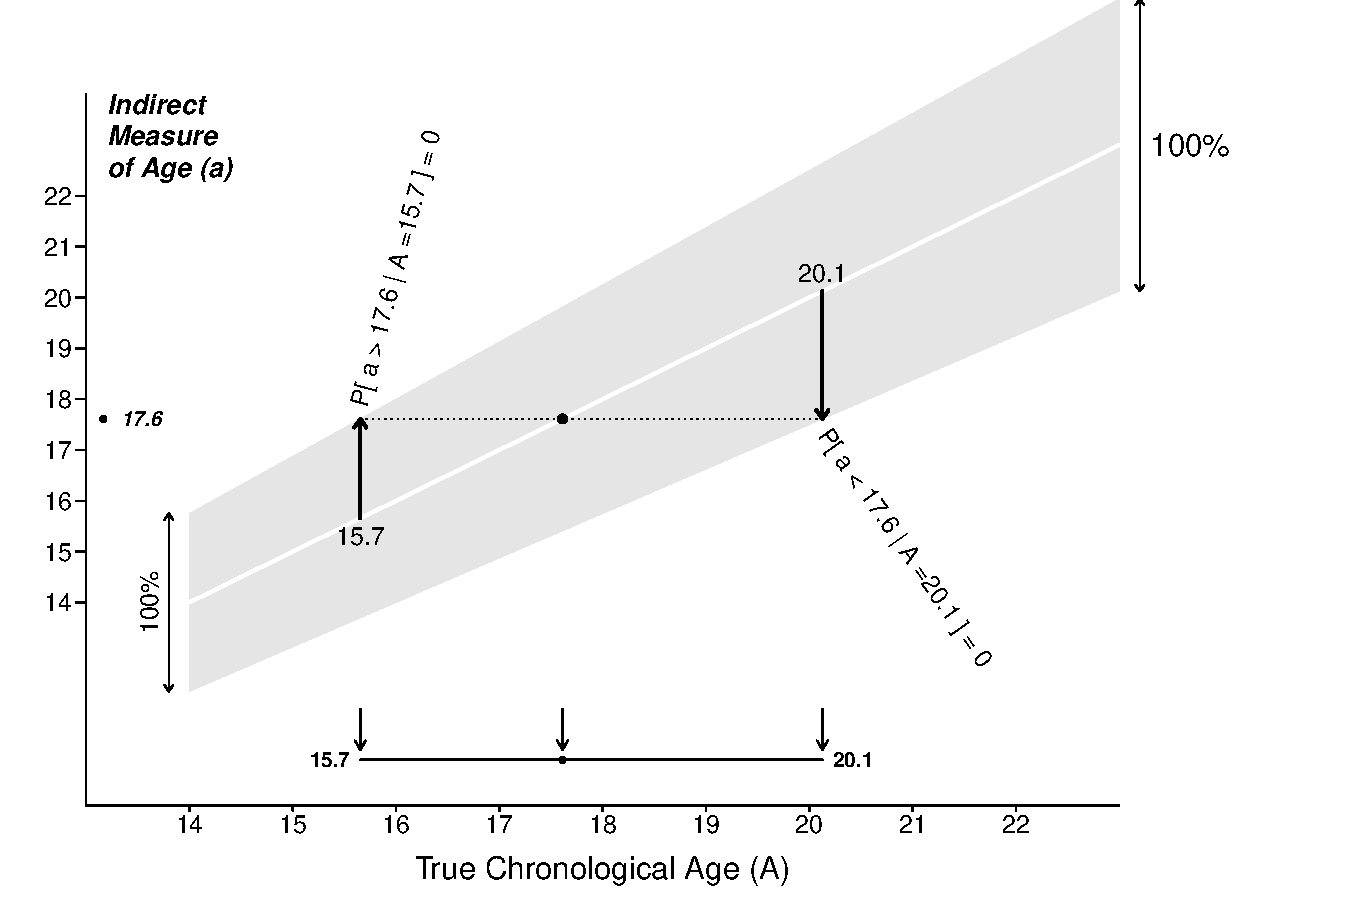
\includegraphics[width=\maxwidth]{figure/unnamed-chunk-2-1} 

}

\caption[100\% Confidence Intervals for a person's chronological age when error distributions (that in this example are wider at the  older ages) are 100\% confined within the shaded ranges]{100\% Confidence Intervals for a person's chronological age when error distributions (that in this example are wider at the  older ages) are 100\% confined within the shaded ranges. }\label{fig:unnamed-chunk-2}
\end{figure}


\end{knitrout}


\end{frame}






\section{Interpreting Frequentist Confidence Intervals}





\begin{frame}{Confidence Interval}
	
	\begin{defm}[Confidence Interval]
		A level $C$ confidence interval for a parameter has two parts:
		\begin{enumerate}
			\item An interval calculated from the data, \underline{usually} of the form $$\textrm{estimate} \pm \textrm{margin of error}$$ where the estimate is a sample statistic and the margin of error represents the accuracy of our guess for the parameter.
			\item A confidence level $C$, which gives the probability that the interval will capture the true parameter value in \textit{different possible samples}. That is, the confidence level is the success rate for the method
		\end{enumerate}
	\end{defm}
	
	%\framedgraphic{6899rule.png}
	
\end{frame}

\frame{\frametitle{Confidence Interval: A simulation study}
	
	\vspace*{-0.1in}
	
	\begin{figure}
		\begin{center}
			\epsfig{figure=CIplots.eps,width=3.2in,height=2.7in}
			\caption{\small{True parameter value is 2 (red line). Each horizontal black line represents a 95\% CI from a sample and contains the true parameter value. The blue CIs do not contain the true parameter value. 95\% of all samples give an interval that contains the population parameter.}}
		\end{center}
	\end{figure}
}





\begin{frame}{Confidence Intervals: we only get one shot}
	\begin{itemize}
		\setlength\itemsep{2em}
		\item In practice, we don't take many simple random samples (``repeated'' samples) to estimate the population parameter $\theta$. \pause 
		\item Because the method has a 95\% success rate, all we need is one simple random sample to compute one CI. 
	\end{itemize}
\end{frame}

\begin{frame}{Interpreting a frequentist confidence interval}
	\begin{itemize}
		\setlength\itemsep{1em}
		\item The confidence level is the success rate of the method that produces the interval. \pause
		\item We don't know whether the 95\% confidence interval from a \underline{particular
			sample} is one of the 95\% that capture $\theta$ (the unknown population parameter), or one of the unlucky 5\% that miss. \pause
		\item To say that we are 95\% confident that the unknown value of $\theta$
		lies between $U$ and $L$ is shorthand for ``We got these numbers using a
		method that gives correct results 95\% of the time.''
	\end{itemize}
\end{frame}

%\frame{\frametitle{Inference for a single population mean} So to
%perform inference, we want an estimator that is unbiased for the
%parameter of interest and that has a relatively small spread (low
%variability or high efficiency). \\ \ \\
%Examples - estimating the population mean $\mu$:
%\begin{itemize}
%\item What is the bias (if any) of $\frac{1}{n}\sum^n_{i=1}(x_i + 1)$?
%\item[] \item What is the bias (if any) of $\frac{1}{n}\sum^n_{i=1}x_i + \frac{1}{n}$?
%\item[] \item Which of the two estimators above would you prefer?
%\end{itemize}
%}


\begin{frame}{More about a frequentist confidence interval}
	
	\begin{itemize}
		\item The confidence level of 95\% has to say something about the sampling procedure: 
		
		\begin{itemize}
			\item The confidence interval depends on the sample. If the sample had come out differently, the confidence interval would have been different. 
			\item With some samples, the interval 'estimate $\pm$ margin of error' does trap the population parameter (the word statisticians use is cover). But with other samples, the interval fails to cover.
		\end{itemize}
		\pause
		\item It's like buying a used car. Sometimes you get a lemon – a confidence interval which doesn't cover the parameter.
		
		\framedgraphiccaption{lemon.jpg}{3 confidence intervals 'chasing' (taking a shot at) the population parameter $P$}
	\end{itemize}
\end{frame}


\begin{frame}{More about a frequentist confidence interval}
	\begin{itemize}
		\setlength\itemsep{2em}
		\item In the frequentist approach, $\theta$ is regarded as a fixed (but unknowable) constant, such as the exact speed of light to an infinite number of digits, or the exact mean depth of the ocean at a given point in time. \pause
		
		\item It doesn't ``fall'' or ``vary around'' any particular values; in contrast you can think of the statistic $\hat{\theta}$ ``falling'' or ``varying around'' the fixed (but unknowable) value of $\theta$
	\end{itemize}
\end{frame}


\begin{frame}{Polling companies}
	\begin{itemize}
		\setlength\itemsep{2em}
		\item Polling companies who say ``polls of this size are accurate to within so many percentage points 19 times out of 20'' are being statistically correct $\to$ they emphasize the \textbf{procedure} rather than what has happened in this specific instance. 
		\item Polling companies (or reporters) who say ``this poll is accurate .. 19
		times out of 20'' are talking statistical nonsense -- this specific poll is either right or wrong. On average 19 polls out of 20 are ``correct''. But this
		poll cannot be right on average 19 times out of 20.
	\end{itemize}
\end{frame}

\frame{\frametitle{Example: Inference for a single population mean} We begin
	with the (unrealistic) assumption that the population variance is
	known.
	\begin{itemize}
		\item Then the true variance of the sample mean is known!
		\item We can use \texttt{mosaic::xpnorm(q = c(-1.96, 1.96))} to find that there is a 95\% chance that a $\mathcal{N}$(0,1) random variable lies within 1.96 
		standard errors of the population mean of the distribution. So then:
		\[ P\left(-1.96 \le \frac{\bar{y}-\mu}{\sigma/\sqrt{n}} \le
		1.96\right) = 0.95 \]
		\item[]
	\end{itemize}
	What does allow us to learn about $\mu$? }

\frame{\frametitle{Example: Inference for a single population mean} We can
	use this probability statement about the standardized version of
	$\bar{y}$ to place bounds on where we think the true mean lies
	by examining the probability that $\bar{y}$ is within
	1.96$\frac{\sigma}{\sqrt{n}}$ of $\mu$. \\ \ \\
	
	$P\left(-1.96 \le \frac{\bar{y}-\mu}{\sigma/\sqrt{n}} \le
	1.96\right)$\\
	\[\begin{array}{ccl} \qquad & = & P\left(-1.96\frac{\sigma}{\sqrt{n}}
	\le \bar{y}-\mu \le +1.96\frac{\sigma}{\sqrt{n}}\right)\\
	\pause
	& = & P\left(-\bar{y}-1.96\frac{\sigma}{\sqrt{n}} \le
	-\mu \le -\bar{y}+1.96\frac{\sigma}{\sqrt{n}}\right)\\ \pause
	& = & P\left(\bar{y}+1.96\frac{\sigma}{\sqrt{n}} \ge
	\mu \ge \bar{y}-1.96\frac{\sigma}{\sqrt{n}}\right)\\ \pause
	& = & P\left(\bar{y}-1.96\frac{\sigma}{\sqrt{n}} \le \mu
	\le \bar{y}+1.96\frac{\sigma}{\sqrt{n}}\right)\\
	& = & 0.95\\
	& & \\
	\end{array}\]
	
	We call the interval
	$\left(\bar{y}-1.96\frac{\sigma}{\sqrt{n}},
	\bar{y}+1.96\frac{\sigma}{\sqrt{n}}\right)$ a \textbf{95\%
		confidence interval} for $\mu$. }

\frame{\frametitle{Example: Inference for a single population mean} So what does the CI allow us
	to learn about $\mu$?? \pause
	
	\begin{itemize}
		\setlength\itemsep{.5em}
		\item In classical (frequentist) statistics, we assume that the population
		mean, $\mu$ is a \textbf{fixed} but unknown value.
		\item With this view, it doesn't make sense to think of $\mu$ as
		having a distribution. Therefore we can't make probability statements about $\mu$. \pause
		\item What about the CI? It is made up of the sample mean
		and other fixed numbers (1.96, the square root of the known sample
		size $n$, and the known standard deviation, $\sigma$).
		\item \textcolor{blue}{\textbf{The CI is a random quantity.}}
		\item Remember: a random quantity is one in which the outcome is not
		known ahead of time. We don't know the lower and upper limits of the
		CI before the sample has been collected since we don't yet know the
		value of the random quantity $\bar{x}$.
	\end{itemize}
	
}

\frame{\frametitle{Example: Inference for a single population mean} So what
	does the CI allow us to learn about $\mu$??
	\begin{itemize}
		\setlength\itemsep{2em}
		\item It tells us that if we repeated this procedure again and again
		(collecting a sample mean, and constructing a 95\% CI), 95\% of the
		time, the CI would \textit{cover} $\mu$. \pause 
		\item That is, with 95\% probability, the \textit{procedure}
		will include the true value of $\mu$. Note that we are making \underline{a probability statement about the CI}, not about the parameter. \pause
		\item Unfortunately, \textcolor{blue}{we do not know whether the true value of $\mu$ is
			contained in the CI in the particular experiment that we have
			performed.}
	\end{itemize}
}


\begin{frame}{Interactive visualization of CIs}
	\Large\href{http://rpsychologist.com/d3/CI/}{http://rpsychologist.com/d3/CI/}
\end{frame}



\begin{frame}[fragile]{Exercise: How deep is the ocean?}
	%\begin{exm}[Confidence intervals in many samples]
	\begin{enumerate}
		\item For your samples of $n=5$ and $n=20$ of depths of the ocean, calculate the
		\begin{enumerate}
			\item sample mean ($\bar{y}$)
			\item standard error of the sample mean ($SE_{\bar{y}}$)
		\end{enumerate}
		\item Calculate the 68\%, 95\% and 99\% confidence intervals (CI) for both samples of $n=5$ and $n=20$.
		\item Enter your results in the \href{https://docs.google.com/spreadsheets/d/1Mnxeq9nQcTdQycZ7S_62fYFiNC5_a3fibsyodzfwO58/edit?usp=sharing}{Google sheet} 
		\item Plot the CIs for each student using the following code:
		
\begin{knitrout}\tiny
\definecolor{shadecolor}{rgb}{0.969, 0.969, 0.969}\color{fgcolor}\begin{kframe}
\begin{alltt}
\hlkwd{plot}\hlstd{(dt}\hlopt{$}\hlstd{Mean.5.depths,} \hlnum{1}\hlopt{:}\hlkwd{nrow}\hlstd{(dt),} \hlkwc{pch}\hlstd{=}\hlnum{20}\hlstd{,}
\hlkwc{xlim}\hlstd{=}\hlkwd{range}\hlstd{(}\hlkwd{pretty}\hlstd{(}\hlkwd{c}\hlstd{(dt}\hlopt{$}\hlstd{lower.mean.5.66, dt}\hlopt{$}\hlstd{upper.mean.5.66))),}
\hlkwc{xlab}\hlstd{=}\hlstr{'Depth of ocean (m)'}\hlstd{,} \hlkwc{ylab}\hlstd{=}\hlstr{'Student (sample)'}\hlstd{,}
\hlkwc{las}\hlstd{=}\hlnum{1}\hlstd{,} \hlkwc{cex.axis}\hlstd{=}\hlnum{0.8}\hlstd{,} \hlkwc{cex}\hlstd{=}\hlnum{1.5}\hlstd{)}
\hlkwd{abline}\hlstd{(}\hlkwc{v} \hlstd{=} \hlnum{3700}\hlstd{,} \hlkwc{lty} \hlstd{=} \hlnum{2}\hlstd{,} \hlkwc{col} \hlstd{=} \hlstr{"red"}\hlstd{,} \hlkwc{lwd} \hlstd{=} \hlnum{2}\hlstd{)}
\hlkwd{segments}\hlstd{(}\hlkwc{x0} \hlstd{= dt}\hlopt{$}\hlstd{lower.mean.5.66,} \hlkwc{x1}\hlstd{=dt}\hlopt{$}\hlstd{upper.mean.5.66,}
\hlkwc{y0} \hlstd{=} \hlnum{1}\hlopt{:}\hlkwd{nrow}\hlstd{(dt),} \hlkwc{lend}\hlstd{=}\hlnum{1}\hlstd{)}
\end{alltt}
\end{kframe}
\end{knitrout}
		
	\end{enumerate}
	%\end{exm}
\end{frame}

\end{document}


